\documentclass[dvisvgm,hypertex,aspectratio=169]{beamer}
\usefonttheme{serif}

\usepackage{animate}

%%%%%%%%%%%%%%%%%%%%%%%%%%%%%%%%%%%%%%%%%%%%%%%%%%%%%%%%%%%%%%%%%%%%%%%%%%%%%%%
% PageDown, PageUp key event handling; navigation symbols
%%%%%%%%%%%%%%%%%%%%%%%%%%%%%%%%%%%%%%%%%%%%%%%%%%%%%%%%%%%%%%%%%%%%%%%%%%%%%%%
\usepackage[totpages]{zref}
\usepackage{atbegshi}
\usepackage{fontawesome}
\setbeamertemplate{navigation symbols}{}
\AtBeginShipout{%
  \AtBeginShipoutAddToBox{%
    \special{dvisvgm:raw
      <defs>
      <script type="text/javascript">
      <![CDATA[
        document.addEventListener('keydown', function(e){
          if(e.key=='PageDown'){
            \ifnum\thepage<\ztotpages
              document.location.replace('\jobname-\the\numexpr\thepage+1\relax.svg');%
            \fi
          }else if(e.key=='PageUp'){
            \ifnum\thepage>1
              document.location.replace('\jobname-\the\numexpr\thepage-1\relax.svg');%
            \fi%
          }
        });
      ]]>
      </script>
      </defs>
    }%
  }%
  \AtBeginShipoutUpperLeftForeground{%
    \raisebox{-\dimexpr\height+0.5ex\relax}[0pt][0pt]{\makebox[\paperwidth][r]{%
      \normalsize\color{structure!40!}%
      \ifnum\thepage>1%
        \href{\jobname-\the\numexpr\thepage-1\relax.svg}{\faArrowLeft}%
      \else%  
        \textcolor{lightgray}{\faArrowLeft}%  
      \fi\hspace{0.5ex}%
      \ifnum\thepage<\ztotpages%
        \href{\jobname-\the\numexpr\thepage+1\relax.svg}{\faArrowRight}%
      \else%
        \textcolor{lightgray}{\faArrowRight}%  
      \fi%
      \hspace{0.5ex}%
    }}%
  }%  
}%
%%%%%%%%%%%%%%%%%%%%%%%%%%%%%%%%%%%%%%%%%%%%%%%%%%%%%%%%%%%%%%%%%%%%%%%%%%%%%%%

%required by PSTricks example
\usepackage[dvipsnames,svgnames]{pstricks}
\usepackage{pst-node,pst-plot,pst-eucl}
\usepackage{pst-solides3d}
\usepackage{multido}
\usepackage[nomessages]{fp}
\usepackage{media4svg}

\AtBeginSection[]
{
  \begin{frame}
    \frametitle{Agenda}
    \tableofcontents[currentsection]
  \end{frame}
}


\setbeamertemplate{footline}[text line]{%
  \parbox{\linewidth}{\vspace*{-8pt}Graph Clustering\hfill\hfill\insertframenumber\,/\,\inserttotalframenumber}}

\title[Graph Clustering]{Graph Clustering}
\author[Georg Grab]{Georg Grab}
\institute[Heidelberg University]{Heidelberg University}
\date{Distributed \& Parallel Algorithms, Summer 2022}

%\includeonlyframes{measuring-clustering-quality-modularity-definition}
%\includeonlyframes{louvain-par-challenge}
\begin{document}

\frame{\titlepage}

\begin{frame}
\frametitle{Agenda}
\tableofcontents
\end{frame}

\section{Basics and Motivation}

\begin{frame}{Graph Clustering: Why?}{}
\begin{figure}
    \includegraphics<1>[scale=0.7]{220523_distparallel_plain.drawio.svg}
    \includegraphics<2>[scale=0.7]{220523_distparallel_output.drawio.svg}
    \caption{\only<1>{Given some input graph...} \only<2>{...group related vertices into \textbf{clusters}.}}
\end{figure}
\end{frame}

\begin{frame}{Motivation: Karate Club Dataset}

Can we detect how this Karate Club will split, \textbf{based on interactions of members}?

\begin{figure}
  \only<1>{\includemedia[width=32em,height=16em,autoplay,muted,embed=false]{}{partial_movie_files/ImportNetworkxGraph/1_draw.mp4}}
  \only<2>{\includemedia[width=32em,height=16em,autoplay,muted,embed=false]{}{partial_movie_files/ImportNetworkxGraph/3_color.mp4}}
  \only<3>{\includemedia[width=32em,height=16em,autoplay,muted,embed=false]{}{partial_movie_files/ImportNetworkxGraph/5_reorder.mp4}}
  \caption{
    \only<1>{\textbf{Vertices} are members, \textbf{edges} are connections between them.} 
    \only<2>{Run a \textbf{clustering algorithm}.}
    \only<3>{Reorder based on clustering.}
    }
\end{figure}
\end{frame}

\section{Measuring Clustering Quality}

\begin{frame}{Measuring Clustering Quality: Modularity (introduction)}

Modularity [Newman et al., 2004], denoted $Q$, is a popular metric used to evaluate a given clustering.
\begin{enumerate}
 \item<1-> $Q \in [-0.5; 1]$
 \item<2-> "Rule of thumb": $Q > 0.3$ means the clustering of the given graph is of decent quality.
 \item<3->{Not without flaws, but still popular}
 \item<4->{Basic idea: compare a graph with a given clustering with a \emph{randomly rewired} version...}
\end{enumerate}

\end{frame}

\begin{frame}{Measuring Clustering Quality: Modularity (intuition)}
\begin{figure}
  \only<1>{\includemedia[width=32em,height=16em,autoplay,muted,embed=false]{}{rewire_edges_start.mp4}}
  \only<2>{\includemedia[width=32em,height=16em,autoplay,muted,embed=false]{}{rewire_edges_rewiring_shortened.mp4}}
  \caption{
    \only<1>{Start with a given clustering} 
    \only<2>{Randomly rewire, preserving vertex degrees.}
    }
\end{figure}
\end{frame}

\begin{frame}[label=measuring-clustering-quality-modularity-definition]{Measuring Clustering Quality: Modularity (definition)}

In the following, let $k_v$ be the degree of vertex $v$. Let $A$ be the adjacency matrix of the graph. Let $c_v$ denote that vertex $v$ belongs to cluster $c_v$.

\begin{enumerate}
 \item<1-> Goal: compare the fraction of edges within clusters with the \emph{expectation} of the same value in a randomly rewired graph.
 \item<2-> Fraction of edges within clusters:

  \begin{equation}
      \frac{1}{2m} \sum_{vw} A_{vw}\ \delta(c_v, c_w)
  \label{eqn:fraction_of_edges_within_cluster}
  \end{equation}

  \item<3-> What can we say about the \emph{probability} of two vertices being connected, knowing only vertex degrees?
  \begin{equation}
    \frac{k_v\ k_w}{2m-1}.
  \label{eqn:randomly_rewired_graph_probabilities}
  \end{equation}

  \item<4-> Putting both together, we get the definition of modularity:
  \begin{equation}
    Q = \frac{1}{2m} \sum_{vw} (A_{vw}\ - \frac{k_v\ k_w}{2m-1}) \delta(c_v, c_w)
  \label{eqn:modularity}
  \end{equation}
\end{enumerate}
\end{frame}

\section{(Parallel) Louvain Algorithm}

\begin{frame}{Louvain Algorithm (serial)}{}
\begin{enumerate}
 \item<1-> Every vertex starts in own cluster. Also assign arbitrary order.
 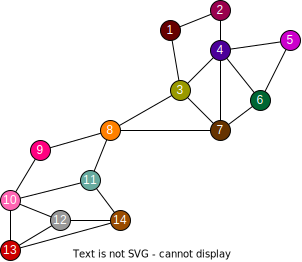
\includegraphics[scale=0.45]{220523_distparallel_louvainstart.drawio.svg}
 \item<2-> Traverse vertices sequentially. For every vertex:
 \begin{enumerate}
   \item<3-> Does clustering get better if the vertex gets assigned to \textbf{neighbor clusters}? ($\Delta Q$)
   \item<4-> \textbf{Assign} vertex to neighbor vertex' cluster that improves clustering the most.
 \end{enumerate}
 \item<5-> Collapse clusters into \emph{Super Nodes}. Repeat till convergence.
\end{enumerate}
\end{frame}

\begin{frame}{How to make this parallel?}
  \begin{itemize}
    \item<1-> Basic idea: traverse vertices \textbf{in parallel} without locks.
    \item<2-> Use a set of heuristics to \textbf{avoid these challenges}:
    \begin{enumerate}
      \item<3-> Nodes moving into their respective clusters \textbf{concurrently}.
      \item<4-> Clustering getting worse due to lacking information.
    \end{enumerate}
  \end{itemize}
\end{frame}

\begin{frame}[label=louvain-par-challenge]{Louvain Algorithm (parallelization challenges)}
  \begin{enumerate}
  \item<1-> Consider thread $b$ is currently on $C_b$ and thread $c$ is on $C_b$:
  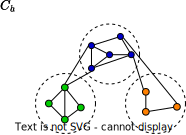
\includegraphics[scale=0.7]{220523_distparallel.drawio.fig1a.svg}

  \item<2-> What actually happens:
  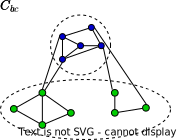
\includegraphics[scale=0.7]{220523_distparallel.drawio.fig1b.svg}
  \end{enumerate}
\end{frame}

\begin{frame}{Louvain Algorithm (parallel heuristic: coloring)}
  \begin{itemize}
    \item<1-> Consider a distance-1 coloring of a graph:
    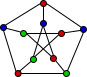
\includegraphics[scale=1.5]{220523_distparallel.drawio.coloring.svg}
    \item<2-> \textbf{Idea:} only process one color at a time in parallel.
    \item<3-> Avoids vertex swaps, but what about negative modularity gain?
  \end{itemize}
\end{frame}

\begin{frame}{Louvain Algorithm (parallel heuristic: minimum label)}
  \begin{itemize}
    \item<1-> How to prevent vertex swapping and negative modularity gain \textbf{initially}?
    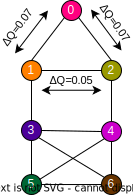
\includegraphics[scale=0.8]{220523_distparallel.drawio.singlet_minimum_label.svg}
    \item<2-> \textbf{Idea:} only execute move if $l(v) < l(w)$.
  \end{itemize}
\end{frame}
\section{(Parallel) Label Propagation}

\begin{frame}{Label Propagation (serial)}{}
\begin{enumerate}
 \item<1-> Every vertex starts in own cluster. Also assign random iteration order.
 \item<2-> Traverse vertices sequentially. For every vertex:
 \begin{enumerate}
   \item<3-> Assign its cluster to the majority of neighbor clusters. Split ties randomly.
 \end{enumerate}
 \item<5-> Repeat this multiple times if necessary. Generate new random iteration order each time.
\end{enumerate}
\end{frame}

\begin{frame}{Label Propagation (intuition)}
\begin{figure}
  \only<1>{\includemedia[width=32em,height=16em,autoplay,muted,embed=false]{}{label_propagation_start.mp4}}
  \only<2>{\includemedia[width=32em,height=16em,autoplay,muted,embed=false]{}{label_propagation.mp4}}
  \caption{
    \only<1>{Vertices start in their own clusters} 
    \only<2>{Iterate, assign to the majority cluster label of neighbors.}
    }
\end{figure}
\end{frame}

\begin{frame}{Label Propagation (discussion)}
\begin{enumerate}
    \item<1-> The serial algorithm is nondeterministic because ties are split randomly.
    \item<2-> It is possible for vertices to change labels indefinitely. 
    \item<3-> \textbf{How to parallelize?} Split vertices evenly, process in parallel.
    \item<4-> We now have randomness for free due to parallelism: assigning random iteration order no longer needed!
    \item<5-> Race conditions will occur, but "might be beneficial"...
\end{enumerate}
\end{frame}

\begin{frame}{Label Propagation (why are race conditions fine?)}
\begin{figure}
  \only<1>{\includemedia[width=32em,height=16em,autoplay,muted,embed=false]{}{label_propagation_sync_update_start.mp4}}
  \only<2>{\includemedia[width=32em,height=16em,autoplay,muted,embed=false]{}{label_propagation_sync_update.mp4}}
  \only<3>{\includemedia[width=32em,height=16em,autoplay,muted,embed=false]{}{label_propagation_bipartite_start.mp4}}
  \only<4>{\includemedia[width=32em,height=16em,autoplay,muted,embed=false]{}{label_propagation_bipartite.mp4}}
  \caption{
    \only<1>{Bipartite Graph with synchronous updating...} 
    \only<2>{...will oscillate indefinitely.}
    \only<3>{Bipartite Graph with \textbf{a}synchronous updating...} 
    \only<4>{...behaves slightly better (at least no oscillations)}
    }
  \label{fig:label-propagation-bipartite}
\end{figure}
\end{frame}
\section{(Distributed) Triangle Counting}

\begin{frame}{What's triangle counting?}{}
\begin{enumerate}
 \item<1-> Quite literally, the count of triangles incident to each vertex
 \begin{figure}
     \includegraphics<1->[scale=0.5]{220621_triangle_count_overview.svg}
 \end{figure}
 \item<2-> Used for computing clustering coefficient, both per-vertex and globally.
 \item<3-> Serial algorithm (boring): for every vertex, check if neighbors are themselves neighbors.
\end{enumerate}
\end{frame}

\begin{frame}{Triangle Counting: What's MapReduce?}{}
\begin{enumerate}
 \item<1-> MapReduce is a programming paradigm for designing distributed algorithms.
 \item<2-> Fundamental Currency: Key-Value tuple: $(k, v)$
 \begin{figure}
     \includegraphics<3->[scale=0.5]{220621_mapreduce_overview.svg}
 \end{figure}
 \item<4-> \textbf{Main Idea:} Map and Reduce operations can be split across multiple compute nodes.
\end{enumerate}
\end{frame}

\begin{frame}[t]{Triangle Counting: MapReduce Algorithm}{}
 \begin{figure}
     \includegraphics<1->[scale=0.25]{220523_surietal_graph_example.svg}
 \end{figure}
 \begin{figure}
     \includegraphics<2->[scale=0.4]{220523_graph_first_stage.svg}
 \end{figure}
 \begin{figure}
     \includegraphics<3->[scale=0.4]{220621_surietal_graph_second_stage.svg}
 \end{figure}
\end{frame}

\begin{frame}{Triangle Counting: Curse of the Last Reducer}
\begin{figure}
     \includegraphics<1->[scale=0.5]{220621_surietal_reducer_completion_times.png}
     \caption{From [Suri et al. 2015]}
\end{figure}
\end{frame}
\section{Discussion}

\begin{frame}{Discussion: Parallel vs. Serial Performance}
\begin{itemize}
\item<1-> Parallel Louvain: 1.45x to 13.07x speedup over serial (measured on several real life datasets)
\item<2-> Parallel Label Propagation: "Unmatched" in execution time, also compared to other parallel algorithms (but no quantitative details vs. serial), \textbf{but} clustering results worse.
\item<3-> Triangle Counting: Successfully processed subset of Twitter (41.7 million user profiles (\textbf{nodes}), 1.47 billion social relations (\textbf{edges}) on a 1636 node compute cluster in 423 minutes.
\end{itemize}
\end{frame}

\begin{frame}{Discussion: Why should you care?}

There are many (parallel) graph clustering algorithms. Why show you these ones?

\begin{itemize}
    \item<1-> Parallel Louvain \& Parallel Label Propagation: implemented in Neo4J $\rightarrow$ mature, used in production everyday.
    \item<2-> Distributed Triangle Counting: raises question of \emph{data skew} present in real life datasets.
\end{itemize}
\end{frame}

\begin{frame}{Discussion: Limitations}
\begin{itemize}
    \item<1-> This barely scratches the surface, there are many (parallel) graph clustering approaches.
    \item<2-> MapReduce (final Algorithm), is declining in popularity. Fails to handle petabyte scale. But "curse of the last reducer" will remain relevant.
    \item<3-> Parallel Label Propagation: Lack of comparison with serial algorithm makes evaluation difficult.
\end{itemize}
\end{frame}

\begin{frame}{}
  \centering \Large
  \emph{Thanks. Questions?}
\end{frame}



\end{document}